\documentclass[11pt]{article}
\usepackage[utf8]{inputenc}
\usepackage[T1]{fontenc}
\usepackage{amsmath}
\usepackage{amsfonts}
\usepackage{amssymb}
\usepackage[version=4]{mhchem}
\usepackage{stmaryrd}
\usepackage{geometry}
\usepackage{graphicx} 
\usepackage{float}
\geometry{a4paper, margin=1in}  
\title{\textbf{Homework Submission}}
\author{}
\date{}


\begin{document}
	
	\maketitle
	
	
	\section*{Math: Question 1 - 30 points}
	
	We are given $\mathrm{n}=7$ observations in $\mathrm{p}=2$ dimensions. For each observation, there is an associated class label.
	
	\begin{center}
		\begin{tabular}{|c|c|c|c|}
			\hline
			Index & $X_{1}$ & $X_{2}$ & $Y$ \\
			\hline
			1 & 3 & 6 & Blue \\
			2 & 2 & 2 & Blue \\
			3 & 4 & 4 & Blue \\
			4 & 1 & 3 & Blue \\
			5 & 2 & 0 & Red \\
			6 & 4 & 2 & Red \\
			7 & 4 & 0 & $\operatorname{Red}$ \\
			\hline
		\end{tabular}
	\end{center}
	
	\begin{itemize}
		\item (a) Sketch the optimal separating hyperplane, and provide the equation for this hyperplane.
	\end{itemize}
	
	
	\begin{figure}[htbp]
		\centering
		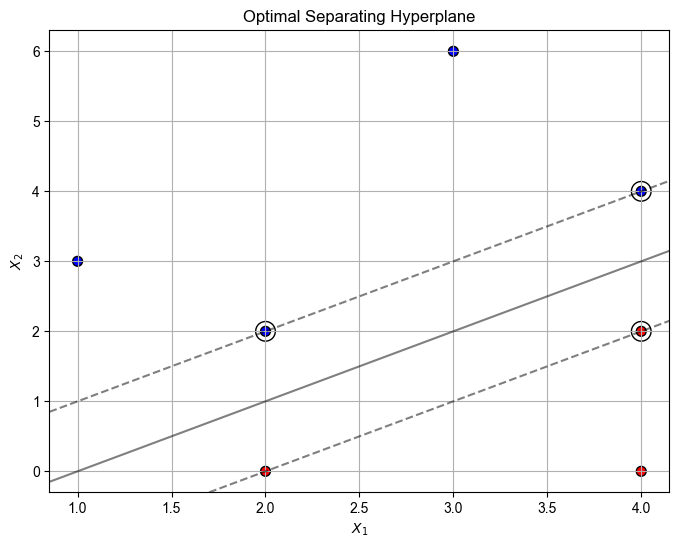
\includegraphics[width=0.7\textwidth]{figures/figure.png}
	\end{figure}
	
	
	The equation of the optimal separating hyperplane is: $X_{1}-X_{2}-1=0$
	
	\begin{itemize}
		\item (b) Describe the classification rule for the maximal margin classifier. It should be something along the lines of "classify to Red if $\beta_{0}+\beta_{1} X_{1}+\beta_{2} X_{2} \geq 0$, and classify to Blue otherwise." Provide the values for $\beta_{0}, \beta_{1}$, and $\beta_{2}$.
	\end{itemize}
	
	The classification rule for the maximal margin classifier is to classify an observation as Red if $\beta_{0}+\beta_{1} X_{1}+\beta_{2} X_{2} \geq 0$ and classify an observation as Blue if $\beta_{0}+\beta_{1} X_{1}+\beta_{2} X_{2}<0$. The values of the coefficients in the hyperplane equation are $\beta_{0}=-1, \beta_{1}=1$, and $\beta_{2}=-1$.
	
	\begin{itemize}
		\item (c) On your sketch, indicate the margin for the maximal margin hyperplane.
	\end{itemize}
	
	It has been shown in Figure 1.
	
	\begin{itemize}
		\item (d) Indicate the support vectors for the maximal margin classifier.
	\end{itemize}
	
	The support vectors for the maximal margin classifier are the observations with coordinates (2, $2$), (4, 4), and (4, 2).
	
	\begin{itemize}
		\item (e) Does a slight movement of the seventh observation affect the maximal margin hyperplane? Justify your answer.
	\end{itemize}
	
	It does not affect the maximal margin hyperplane because it is not a support vector, and its movement does not change the position of the existing support vectors.
	
	\begin{itemize}
		\item (f) Draw an alternative hyperplane that is not the optimal separating hyperplane, and provide the equation for this hyperplane.
	\end{itemize}
	
	
	\begin{figure}[H]
		\centering
		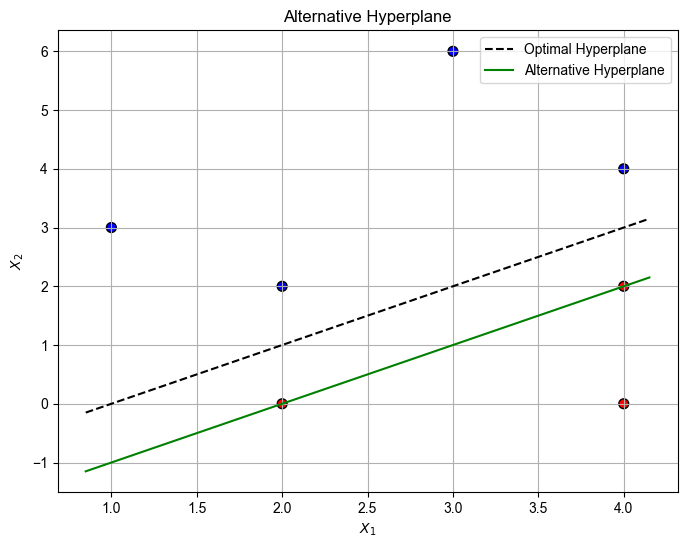
\includegraphics[width=0.7\textwidth]{figures/figure1.png}
	\end{figure}
	
	
	An alternative hyperplane that separates the classes but is not optimal is given by the equation: $-X_{1}+X_{2}+2=0$
	
	\begin{itemize}
		\item (g) Draw an additional observation on the plot so that the two classes are no longer separable by a hyperplane.
	\end{itemize}
	
	
	\begin{figure}[H]
		\centering
		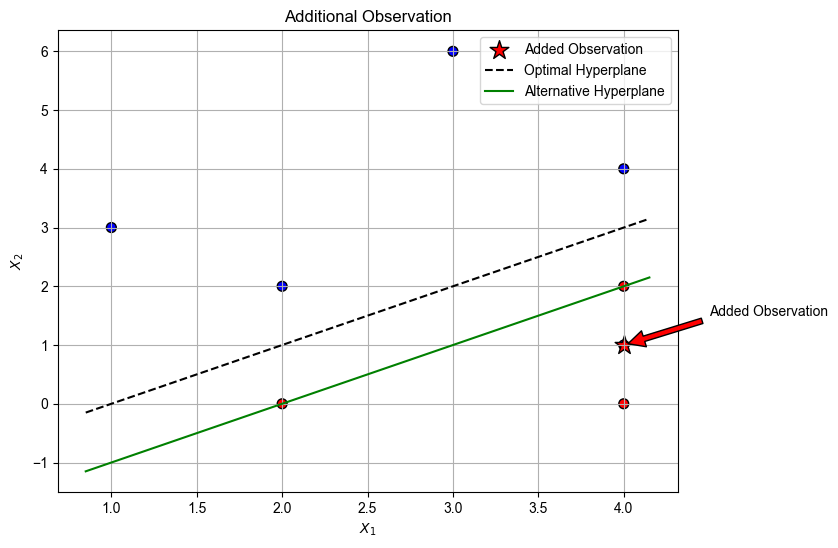
\includegraphics[width=0.9\textwidth]{figures/figure2.png}
	\end{figure}
	
	
	A new observation with coordinates $(4,1)$ and assigning it to the Blue class, the two classes become no longer separable by a hyperplane. This new point lies within the cluster of Red points, making it impossible for a single hyperplane to perfectly separate the Blue and Red classes without misclassification.
	
	\section*{Math: Question 2 - 20 points}
	
	Assume that we have a training data with four samples, 2 features and 2 classes. The positive examples are $(1,1)$ and $(-1,-1)$. The negative examples are $(1,-1)$ and $(-1,1)$.
	
	\begin{itemize}
		\item (a) Draw a table that represents this training set. What is the shape of $X$ and $y$?
		\item (a.bonus) The table you just drew is called a truth table. Do you know the logic gate representing this truth table?
	\end{itemize}
	
	\begin{center}
		\begin{tabular}{|c|c|c|}
			\hline
			$x_{1}$ & $x_{2}$ & $y$ \\
			\hline
			1 & 1 & 1 \\
			-1 & -1 & 1 \\
			1 & -1 & -1 \\
			-1 & 1 & -1 \\
			\hline
		\end{tabular}
	\end{center}
	
	The shape of $\mathrm{X}$ is $(4 \times 2)$, as there are 4 samples and each sample has 2 features. The shape of $\mathrm{y}$ is $(4 \times 1)$, as there are 4 samples and each sample has a corresponding label.
	
	The truth table represents the XOR (exclusive OR) logic gate, where the output is true if and only if the inputs are different.
	
	\begin{itemize}
		\item (b) Draw these four points on $x-y$ plane. Are these points linearly separable?
	\end{itemize}
	
	
	\begin{figure}[H]
		\centering
		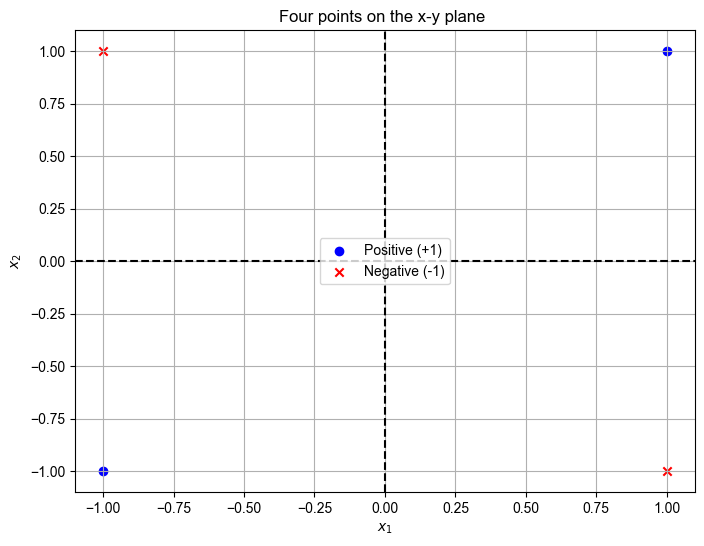
\includegraphics[width=0.7\textwidth]{figures/figure3.png}
	\end{figure}
	
	
	The four points are plotted on the $x-y$ plane as shown in the figure above. It can be found that the points are not linearly separable in the original $2D$ space, as there is no single straight line that can separate the positive examples from the negative examples.
	
	\begin{itemize}
		\item (c) Consider the feature transformation $\phi(x)=\left[x_{1}, x_{2}, x_{1} x_{2}\right]$, where $x_{1}$ and $x_{2}$ are, respectively, the first and second coordinates of a generic example $x$. Draw these four points when transformed by the function $\phi(x)$. Are these four transformed points now linearly separable?
	\end{itemize}
	
	
	\begin{figure}[H]
		\centering
		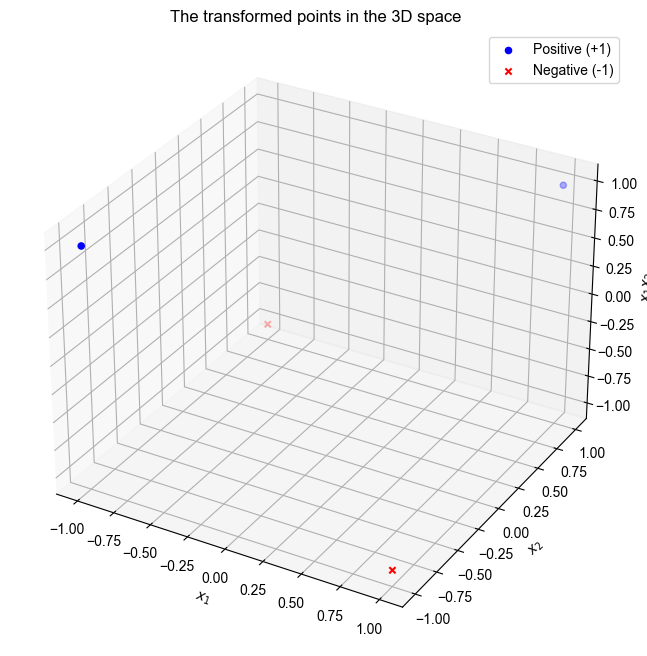
\includegraphics[width=0.7\textwidth]{figures/figure4.png}
	\end{figure}
	
	
	After applying the feature transformation $\phi(x)=\left[x_{1}, x_{2}, x_{1} x_{2}\right]$, the points are mapped into a $3D$ space. In this new space, the transformed points become linearly separable, as there exists a plane that can perfectly separate the positive examples from the negative examples.
	
	\begin{itemize}
		\item (d) What is the margin size after the transformation? Which points are support vectors?
	\end{itemize}
	
	After applying the feature transformation, all four transformed points have an equal distance to the optimal separating hyperplane. They all contribute to defining the maximum margin between the two classes.
	
	\begin{center}
		\begin{tabular}{|c|c|c|c|}
			\hline
			$x_{1}$ & $x_{2}$ & $x_{1} x_{2}$ & Support Vector \\
			\hline
			1 & 1 & 1 & Yes \\
			-1 & -1 & 1 & Yes \\
			1 & -1 & -1 & Yes \\
			-1 & 1 & -1 & Yes \\
			\hline
		\end{tabular}
	\end{center}
	
	Since all points are support vectors, it demonstrates the perfect linear separability achieved after the feature transformation. The margin size is calculated to be 2.0, based on the distance between the support vectors and the separating hyperplane.
	
\end{document}

